\section{Finite Volumenverfahren für Erhaltungsgleichungen in einer Dimension}
\begin{frame}
\frametitle{Finite Volumenverfahren}
\begin{align}
\underbrace{\partial _t u(x,t)}_{\text{Euler}} + \underbrace{\partial _xf(u(x,t),x,t)}_{\text{Satz v. Gauß}} = 0
\end{align}
Lsg:
\begin{align}
u_i^{n+1}:=u_i^n+\frac{\Delta t}{h} (s(u_i^n,(x_i+x_{i+1})/2,t_n)-g(u_{i-1}^n,u_i^n,-1;x_i,t_n)\nonumber \\
+g(u_i^n,u_{i+1}^n,1;x_{i+1},t_n))
\end{align}
+ geeignete Randwerte.
\end{frame}
\begin{frame}
\frametitle{Anschauliches Beispiel}
\begin{figure}
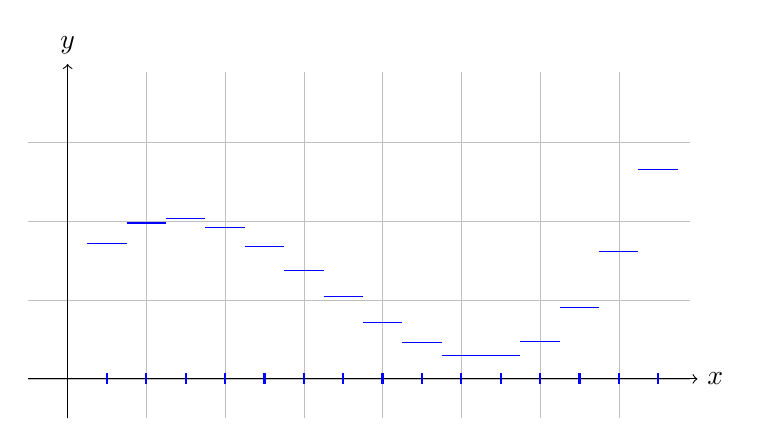
\begin{tikzpicture}[domain=-4:4]
\draw[very thin,color=lightgray] (-0.5, -.5) grid (7.9, 3.9);
\draw[->] (-.5,0) -- (8, 0) node[right] {$x$};
\draw[->] (0,-.5) -- (0, 4) node[above] {$y$};
\draw plot [shift={(4,0)}, samples=50, smooth] function {0.6*(0.1*(x-1)**3 + 
0.5*(x-1)**2 - 
0.3*(x-1) + 0.5)};

\foreach \x in {0.5, 1, ..., 7.9}
{
	\draw[color=blue, thick, shift={(\x, 0)}] (0, 2pt) -- (0pt, -2pt);
	\draw[shift={(\x, {0.6*(0.1*(\x -5)^3 + 0.5*(\x -5)^2 - 0.3*(\x -5) + 0.5)  
	})}, color=blue ] (-0.25, 0) -- (.25, 0);
}

\end{tikzpicture}
\caption{}
\end{figure}
\end{frame}
\begin{frame}
\frametitle{Beispiel: linearer Transport}
$\Omega:=\left[0, 1\right]$, $T:=2$ und Anfangswerte:
\begin{align}
u^0(x):=\left\{\begin{array}{ll} 1, & 0{,}5\leq x \leq 0{,}75 \\
0, & \text{sonst}\end{array}\right.
\end{align}
\begin{align}
f(u,x,t)&:=v\cdot u\\
s(u,x,t)&:=0
\end{align}
und periodischen Randwerten
\end{frame}
\begin{frame}
\frametitle{Simulation des lin. Transports}
\begin{minipage}[t]{0.48\linewidth}
\begin{figure}
\centering
\includegraphics[width=1.\linewidth]{../img/transport_0}
\caption{Anfangswerte des lin. Transports.}
\label{fig:transport_0}
\end{figure}
\end{minipage}
\begin{minipage}[t]{0.5\linewidth}
\begin{figure}
\centering
\includegraphics[width=1.\linewidth]{../img/transport_55}
\caption{lin. Transport mit period. Randwerten}
\label{fig:transport_55}
\end{figure}

\end{minipage}
\end{frame}